\documentclass{article}
\usepackage[utf8]{inputenc}
\usepackage{amsmath}
\usepackage{graphicx}



\title{Compound-Uniswap Liquidator V1 Design Doc}
\author{Jiggaboo Jones}
\date{\today}

\begin{document}

\maketitle
\begin{abstract}

  This system liquidates underwater accounts on Compound. A webserver pulls data from multiple sources to calculate the Revenue of liquidating
  an account, then a transaction is submitted to a smart contract which bundles some actions together to create a pure revenue transaction.
  The transaction calls Uniswap for a flash loan, then it uses the newly borrowed tokens to liquidate a loan on Compound, next it swaps the 
  tokens it seized in the liquidation back to the tokens it took out the flash loan in and pays back the flash loan. Finally it does some checks
  to make sure it hasn't lost money in the transaction and reverts the whole process if it has lost money. 
  \\

  This whole process ensures that all
  transactions that do not fail will only make money, that is to say they are \emph{Pure Revenue Transactions}. The system can only lose small amounts of
  money by paying transaction fees on transactions that revert.

\end{abstract}

\section*{Architecture}
\begin{align*}
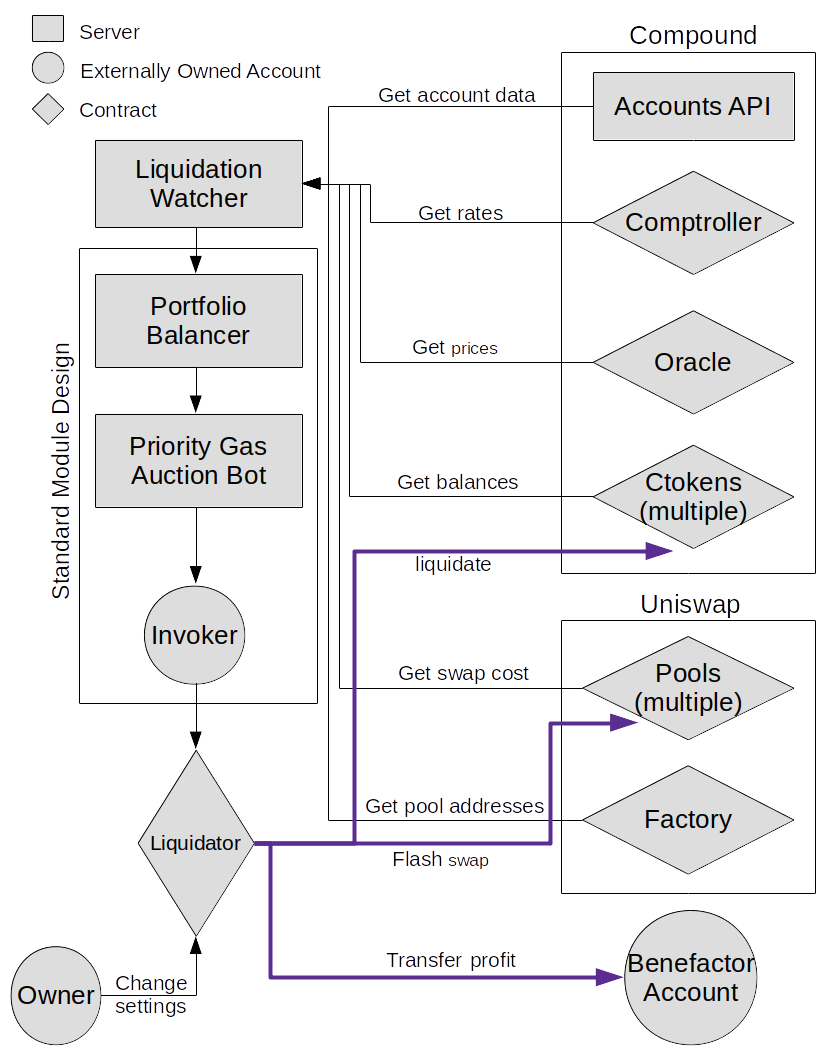
\includegraphics[width=\linewidth]{../Resources/overall_architecture.png}
\end{align*}
\pagebreak


\section*{In Depth Breakdown}
  \subsection*{Liquidation Watcher}
  The Liquidation Watcher watches the block chain for liquidations. It pulls accounts sorted by collateralization from compound's api and calculates the revenue
  from liquidating them in order of least collateralized first (after checking to make sure they are not dust). If it finds an account it can liquidate it then passes
  information to the Transaction Handler in the following JSON format:
  \begin{verbatim}
    {
      String: ethRevenue //Eth Revenue from swapping (in wei),
      String: ethCost //from not swapping (in wei),
      String: tokenRevenue //from not swapping (in atomic),
      String: liquidateAddress //The address of the account to liquidate,
      String: repayToken //letter code (ETH, REP, DAI,...),
      String: seizeToken //letter code of CToken (CETH, CREP, CDAI,...),
      String: repayAmount //The amount of token being repaid (in atomic)
    }
  \end{verbatim}
  \subsection*{Transaction Handler}
  See Transaction handler Documented separately for in depth detail.
  \\
  The Transaction handler decides whether or not to swap tokens based on a portfolio balancer. It also conducts priority gas auctions to
  get the most transactions through at the lowest price. The initial version of this liquidator will run without any portfolio balancing and a
  simple blind raise strategy for the priority gas auction. Other components in this system are designed with these additional features in mind though.
  \pagebreak
  \subsection*{Liquidator}
  The liquidator grants permissions to 3 accounts: Invoker, Owner, and Benefactor.
  The Owner can change the liquidator's settings. The Invoker can call liquidations. The Benefactor can withdraw funds.
  \\
  Liquidation consists of the following steps:
  \begin{itemize}
    \item The Invoker calls the liquidate function
    \item The Liquidator notes it's current balances
    \item The Liquidator gets a flash loan from Uniswap
    \item The Liquidator uses the loan to liquidate the account passed in
    \item The Liquidator seizes CTokens in a different currency as collateral
    \item The Liquidator redeems CTokens for their underlying token (or not if we omit swapping)
    \item The Liquidator repays Uniswap with the redeemed tokens (or with its own balance of the original if we omit swapping)
    \item The Liquidator compares its new balance to its old balance and reverts if it lost money
    \item A gas token optimization is called if the gas price was sufficiently high
  \end{itemize}

  \pagebreak

  \section*{Variable Definitions}
  \begin{itemize}
    \item[$R$ :] Revenue from a successful transaction (measured in ETH), derived from formula below
    \item[$T_{s}$ :] Tokens seized in liquidation, derived from formula below
    \item[$T_{r}$ :] Tokens repaid in liquidation, derived from formula below
    \item[$I$ :] Liquidation incentive. The discount on tokens seized in liquidation, pulled from \emph{Comptroller:liquidationIncentiveMantissa()} (scaled by 1e18)
    \item[$C$ :] Close factor. The percent of an accounts borrowed tokens that can be liquidated in a single transaction, pulled from \emph{Comptroller:closeFactorMantissa()} (scaled by 1e18)
    \item[$P_{s}$ :] Price of seized token in ETH, pulled from \emph{PriceOracle:getUnderlyingPrice(tokenAddress)} (scaled by 1e18)
    \item[$P_{r}$ :] Price of repaid token in ETH, pulled from \emph{PriceOracle:getUnderlyingPrice(tokenAddress)} (scaled by 1e18)
    \item[$L_{b}$ :] Largest borrowed asset in ETH, calculated by calling \emph{CToken:borrowBalanceCurrent(accountAddress)} on each CToken and \emph{PriceOracle:getUnderlyingPrice(tokenAddress)} to calculated the largest position in ETH
    \item[$L_{c}$ :] Largest collateral asset in ETH, calculated by calling \emph{Comptroller:getAssetsIn(accountAddress)} to see which assets are used as collateral, and then measuring each one by checking the balances of each CToken that account is entered into
    \item[$Q$ :] Available flash swap liquidity, pulled from \emph{UniswapPair:getReserves} 
    \item[$f_{u}(T_{r})$ :] Uniswap cost function. Always takes $T_{r}$ as input, available through the uniswap SDK 
  \end{itemize}

  \section*{Formula Definitions}
  \begin{itemize}
    \item[]{\Large $R = (T_{s} - f_{u}(T{r})) * P_{s}$}
    \item[]{\Large $T_{s} = \frac{I * P_{r} * T_{r}}{P_{s}}$}
    \item[]{\Large $T_{r} = \begin{cases} Q, & T_{r} \leq Q \\\frac{L_{c} * P_{s}}{P_{r} * I}, & L_{b} * C * I > L_{c} \\L_{b} * C * I, & L_{b} * C * I \leq L_{c}\end{cases}$}
  \end{itemize}
\end{document}